\documentclass[review]{elsarticle}

\usepackage{graphics, float, url}
\usepackage{graphicx}
\usepackage{subcaption}
\usepackage{lineno,hyperref}
\usepackage{mathtools}
\usepackage{multirow}
\usepackage{adjustbox}
\usepackage{chngpage}
\usepackage{setspace}
\usepackage{amsfonts}
\usepackage{subcaption}
\usepackage{float}
\usepackage[ruled, lined, onelanguage, linesnumbered]{algorithm2e}
\usepackage[usenames,dvipsnames,svgnames,table]{xcolor}
\newcommand{\myfloatalign}{\centering}
\modulolinenumbers[5]

\usepackage{epstopdf}
\epstopdfDeclareGraphicsRule{.tiff}{png}{.png}{convert #1 \OutputFile}
\AppendGraphicsExtensions{.tiff}

\journal{Applied Soft Computing}

%%%%%%%%%%%%%%%%%%%%%%%
%% Elsevier bibliography styles
%%%%%%%%%%%%%%%%%%%%%%%
%% To change the style, put a % in front of the second line of the current style and
%% remove the % from the second line of the style you would like to use.
%%%%%%%%%%%%%%%%%%%%%%%

%% Numbered
%\bibliographystyle{model1-num-names}

%% Numbered without titles
%\bibliographystyle{model1a-num-names}

%% Harvard
%\bibliographystyle{model2-names.bst}\biboptions{authoryear}

%% Vancouver numbered
%\usepackage{numcompress}\bibliographystyle{model3-num-names}

%% Vancouver name/year
%\usepackage{numcompress}\bibliographystyle{model4-names}\biboptions{authoryear}

%% APA style
%\bibliographystyle{model5-names}\biboptions{authoryear}

%% AMA style
%\usepackage{numcompress}\bibliographystyle{model6-num-names}

%% `Elsevier LaTeX' style
\bibliographystyle{elsarticle-num}
%%%%%%%%%%%%%%%%%%%%%%%
\newtheorem{definition}{Definition}
\begin{document}

\begin{frontmatter}

\title{Enhancing instance-level constrained clustering through differential evolution}

\author[mymainaddress]{Germ\'an Gonz\'alez-Almagro\corref{mycorrespondingauthor}}
\cortext[mycorrespondingauthor]{Corresponding author}
\ead{germangalmagro@ugr.es}

\author[mymainaddress]{Juli\'an Luengo}

\author[mysecondaddress]{Jos\'e-Ram\'on Cano}

\author[mymainaddress]{Salvador Garc\'ia}

\address[mymainaddress]{DaSCI Andalusian Institute of Data Science and Computational Intelligence, University of Granada, Spain}

\address[mysecondaddress]{Dept. of Computer Science, EPS of Linares, University of Ja\'en, Campus Cient\'ifico Tecnol\'ogico de Linares, Cintur\'on Sur S/N, Linares 23700, Ja\'en, Spain}

\begin{abstract}
Clustering has always been a powerful tool in knowledge discovery. Traditionally unsupervised, it received renewed attention when it was shown to produce better results when provided with new types of information, thus leading to a new kind of semi-supervised learning: constrained clustering. This technique is a generalization of traditional clustering that considers additional information encoded by constraints. Constraints can be given in the form of instance-level must-link and cannot-link constraints, in which this paper focuses on. We propose the first application of Differential Evolution to the constrained clustering problem, which has proven to produce a better exploration-exploitation trade-off when comparing with previous approaches. We will compare the results obtained by this proposal to those obtained by previous nature-inspired techniques and by some of the state-of-the-art algorithms on 25 datasets with incremental levels of constraint-based information, supporting our conclusions with the aid of Bayesian statistical tests.
\end{abstract}

\begin{keyword}
constrained clustering, instance-level, must-link, cannot-link, genetic algorithm, differential evolution, Bayesian statistical tests.
\end{keyword}

\end{frontmatter}

\linenumbers

\section{Introduction} \label{sec:Intro}

One of the most widely known and studied data analysis problems is clustering. It is one of the most successful methods in the field of unsupervised learning, where there is no supervision on how the information should be handled. Clustering has been able to provide solutions in a large number of knowledge fields, such as, marketing, banking, psychology, psychiatry, astronomy, archaeology, genetics,\cite{Everitt:2009:CA:1538772} cartographic labeling \cite{araujo2019improving} and image segmentation in various fields, ranging from general applications \cite{wang2018non} to very specific ones such as in medicine \cite{verma2016improved, aparajeeta2016modified}.

In the literature, clustering methods are often divided into two subsets: partitional clustering and hierarchical clustering. In hierarchical clustering the result is not a partition of the data with a certain number of clusters---as in partitional clustering---, but instead a dendrogram in which there are partitions that include from the whole dataset to particular individuals \cite{Everitt:2009:CA:1538772}. A representative example of partitional clustering is the widely studied and well-known algorithm K-means \cite{wu2009top}, while for hierarchical clustering the CURE method should be highlighted \cite{guha1998cure}. In this paper we will focus on partitional clustering.

We can define partitional clustering as the task of grouping the instances of a dataset into $k$ clusters, so that new information can be extracted from them. A dataset $X$ is composed of $n$ instances, each one of them described by $d$ features. More formally, $X = \{x_1, \cdots, x_n\}$, with the $i$th instance noted as $x_i = (x_{[i,1]}, \cdots, x_{[i,u]})$. A typical clustering algorithm assigns a class label $l_i$ to each instance $x_i \in X$. As a result, we obtain the set of labels $L = \{l_1, \cdots, l_n\}$, with $l_i \in \{1, \cdots, k\}$, that effectively splits $X$ into $k$ non-overlapping clusters $c_i$ to form a partition called $C$. The criterion used to assign an instance to a given cluster is the similarity to the rest of elements in that cluster, and the dissimilarity to the rest of instances of the dataset, which can be obtained with some kind of distance measurement $d(\cdot, \cdot)$ \cite{jain1999data}.

Semi-supervised learning (SSL) is a machine learning paradigm that arises from adding incomplete information to unsupervised learning. We can divide SSL methods into two broad categories according to their objective: semi-supervised classification and semi-supervised clustering \cite{chapelle2009semi}. The first method has partial information about the labels, so it tries to minimize the error based on them while taking into account the distribution of unlabeled instances. The second tries to obtain better defined clusters incorporating background information to the clustering process, this is known as constrained clustering and is the main subject of the study presented in this paper \cite{triguero2015self}. 

Constrained clustering is an SSL learning method whose goal is to find a partition of the dataset that meets the proper characteristics of a clustering method result, in addition to satisfying a certain constraint set. It has been successfully applied in many knowledge fields, among which it is worth mentioning: advanced robotics applications \cite{davidson2005clustering, semnani2016constrained}, applied marketing \cite{seret2014new}, obstructive sleep apnea analysis \cite{mai2018evolutionary}, handwritten digits classification \cite{li2015scalable}, Internet traffic classification \cite{wang2014internet}, electoral district designing, \cite{brieden2017constrained}, and lane finding in GPS data \cite{wagstaff2001constrained} among others.

Constraints can be understood in different ways, resulting in three main types of constrained clustering: cluster-level \cite{bradley2000constrained}, instance-level \cite{davidson2007survey} and feature-level constrained clustering \cite{schmidt2011clustering}. Moreover, hybrid approaches which try to integrate different types of constraints have also been proposed \cite{wang2010clustering}. 

In particular, we can find in the literature two types of instance-level constraints: pairwise constraints and distance-based constraints. In one hand, pairwise constraints tell us if two specific instances of a dataset must be placed in the same or in different clusters, resulting in Must-link (ML) and Cannot-link (CL) constraints respectively. On the other hand, distance-based constraints do not involve specific instances, but tell us if instances must be placed in the same or in different clusters based on a given distance measure \cite{davidson2007survey}. This paper focuses on pairwise instance-level constraints (ML and CL), which will be discussed later in Section \ref{sec:BackCC}.

Regarding the degree to which the constraints have to be satisfied, we can make a distinction between the concepts of hard \cite{wagstaff2001constrained} and soft \cite{law2004clustering} constraints. Hard constraints must necessarily be satisfied in the output partition of any algorithm that makes use of them, while soft constraints are taken as a strong guide for the algorithm that uses them but can be partially satisfied in the output partition \cite{seret2014new}. For the purposes of this paper, we will employ the latter.

Finding the optimal partition in a dataset, with respect to any kind of reasonable criteria, is known to be a $\mathbf{NP}$-hard problem. Therefore, the incorporation of constraints may modify the complexity of the clustering problem, depending on the type of constraints used. As we will study in more depth in Section \ref{sec:BackFeas}, the use of ML and CL constraints makes the constrained clustering problem $\mathbf{NP}$-complete \cite{davidson2005clustering}.

The constrained clustering problem can be formulated in terms of optimization, so that we can apply various optimization techniques to solve it. As mentioned earlier, it is a difficult problem to solve, so nature-inspired techniques are presented as a promising option to find quality approximate solutions. Nature is the best example of adaptive problem solving since it can apply an optimal strategy suited for each natural phenomenon \cite{fausto2019ants}. Nature-inspired algorithms are designed to emulate natural optimization phenomena, such as evolution, collective behavior of animals, physics laws or even human being-related processes. There have been attempts to solve the constrained clustering problem with nature-inspired algorithms, such as the adaptation of the Biased Random-key Genetic Algorithm (BRKGA) presented in \cite{de2017comparison}. Swarm-based methods have also been applied to constrained clustering, such as the one presented in \cite{xu2013improving}.

Differential Evolution (DE) is an evolution-based algorithm that has proven to be excellent in real-domain problem solving \cite{das2011differential}. In this paper we propose the first DE application to find quality solutions for the constrained clustering problem. In particular, we will take as basis for our proposal one of the DE variants which showed excellent behavior in worldwide competitions, known as SHADE \cite{molina2018insight}. We will make use of the Random-key concept from BRKGA, along with proposing a new fitness function, to build the already mentioned DE variant. We will properly compare the results obtained by our new method with previous nature-inspired algorithms, as well as with the constrained clustering state-of-the-art.

Regarding the organization of this paper, Section \ref{sec:background} reviews the existing knowledge concerning constrained clustering and DE. In Section \ref{sec:brkga} the BRKGA algorithm and its adaptation for constrained clustering will be briefly reviewed. Afterward, the SHADE variant of DE algorithm will be presented in Section \ref{sec:SHADE}. In Section \ref{sec:SHADEadapt} the scheme that allow us to apply SHADE to constrained clustering, including the proposal of a new fitness function, will be presented. Sections from \ref{sec:expSetup} to \ref{sec:analisis} present the experimental setup, results and their analysis respectively. Finally, in Section \ref{sec:conclusiones} conclusions are discussed.

\section{Background} \label{sec:background}

In this section we present the background knowledge concerning constrained clustering (Section \ref{sec:BackCC}), its computational complexity (Section \ref{sec:BackFeas}) and a brief description of some of the state-of-the-art methods for constrained clustering (Section \ref{sec:BackSOTA}). We will also present the basis of the DE optimization method (Section \ref{sec:BackDE}).

\subsection{Constrained Clustering} \label{sec:BackCC}

In most clustering applications it is common to have some kind of information about the dataset to be analyzed. In pairwise instance-level constrained clustering this information is given in the form of pairs of instances. A constraint states whether the instances which it refers to must, or must not, be assigned to the same cluster. It is possible to obtain a better result by using this type of information than by using completely unsupervised clustering algorithms. We can now formalize the two type of constraints mentioned: 

\begin{itemize}

	\item Must-link constraints $C_=(x_i,x_j)$: instances $x_i$ and $x_j$ from $X$ must be placed in the same cluster.

	\item Cannot-link constraints $C_{\neq}(x_i,x_j)$: instances $x_i$ and $x_j$ from $X$ cannot be assigned to the same cluster.

\end{itemize}

The goal of constrained clustering is to find a partition (or clustering) of $k$ clusters $C = \{c_1, \cdots, c_k\}$ of the dataset $X$ that ideally satisfies all constraints in the constraint set. As in the original clustering problem, it must be fulfilled that the sum of instances in each cluster $c_i$ is equal to the number of instances in $X$, which we have defined as $n = |X| = \sum_{i = 1}^{k} |c_i|$.

Knowing how a constraint is defined, ML constraints are an example of an equivalence relation; therefore, ML constraints are reflexive, transitive and symmetric. This way, given constraints $C_=(x_a,x_b)$ and $C_=(x_b,x_c)$ then $C_=(x_a,x_c)$ is verified. In addition, if $x_a \in c_i$ and $x_b \in c_j$ are related by $C_=(x_a,x_b)$, then $C_=(x_c,x_d)$ is verified for any $x_c \in c_i$ and $x_d \in c_j$ \cite{davidson2007survey}.

It can also be proven that CL constraints do not constitute an equivalence relation. However, analogously, given $x_a \in c_i$ and $x_b \in c_j$, and the constraint $C_{\neq}(x_a,x_b)$, then it is also true that $C_{\neq}(x_c,x_d)$ for any $x_c \in c_i$ and $x_d \in c_j$ \cite{davidson2007survey}.

\subsection{The Feasibility Problem} \label{sec:BackFeas}

Given that constrained clustering adds a new element to the clustering problem, we must consider how this element affects the complexity of the problem. The feasibility problem for non-hierarchical instance-level constrained clustering was defined in \cite{davidson2005clustering} as in Definition \ref{def1}.

\begin{definition}

	\textbf{Feasibility Problem}: given a dataset $X$, a constraint set $CS$, and the bounds on the number of clusters $k_l \leq k \leq k_u$, does there exist a partition $C$ of $X$ with $k$ clusters such that all constraints in $CS$ are satisfied? \cite{davidson2005clustering}
	\label{def1}

\end{definition}

In \cite{davidson2005clustering} it is proven that, when $k_l = 1$ and $k_u \ge 3$, the feasibility problem for constrained clustering is $\mathbf{NP}$-complete, by reducing it from the Graph K-Colorability problem (it is also proven that it is not harder, so both have the same complexity). Table \ref{tab:feasibility} shows the complexity of the feasibility for different types of constraints.

\begin{table}[!h]
	\centering
	%\setlength{\arrayrulewidth}{1mm}
	\setlength{\tabcolsep}{7pt}
	\renewcommand{\arraystretch}{1.2}
	%\resizebox{\textwidth}{!}{
		\begin{tabular}{c c}
			\hline
			Constraints & Complexity \\
			\hline
			Must-Link & $\mathbf{P}$\\
			Cannot-Link & $\mathbf{NP}$-complete\\
			ML and CL & $\mathbf{NP}$-complete\\
			\hline

		\end{tabular}%}
	\caption{Feasibility problem complexity \cite{davidson2005clustering}.}
	\label{tab:feasibility}
\end{table}

These complexity results show that the feasibility problem with CL constraints is intractable and hence constrained clustering is intractable too. For more details on the complexity of constrained clustering see \cite{davidson2005clustering}.

Intractable problems are hard to solve with deterministic and exact methods. That is the reason why nature-inspired algorithms constitute good approaches to find quality solutions to the constrained clustering problem.

\subsection{State-of-the-art Methods} \label{sec:BackSOTA}

The first adaptation of a classic clustering method for constrained clustering was proposed in \cite{wagstaff2001constrained}. It involved modifying the widely studied K-means algorithm to take into account instance-level constraints: the already known ML and CL. This method was named COP-kmeans, it introduces a modification to the assignation rule of instances to clusters of the K-means algorithm so that an instance can be assigned to a cluster only if the assignment does not violate any constraint.

In \cite{antoine2012cecm} Constrained Evidential c-means (CECM), a variant of the Evidential c-means (ECM \cite{masson2008ecm}) algorithm is proposed, within the fuzzy clustering family of methods. The particularity of this algorithm is that the membership of instances to a cluster is defined by a probabilistic belief function. This method redefines constraints from the point of view of belief functions and includes them in the fitness function.

A modification of the Constrained Vector Quantization Error algorithm (CVQE \cite{davidson2005clustering}) is proposed in \cite{pelleg2007k}. The CVQE algorithm proved to produce high quality results, at the cost of a very high computational complexity. Linear CVQE (LCVQE) introduces a modification of the cost function of CVQE to make it more intuitive and less computationally complex. The experimentation resulted in a dramatic improvement of clustering quality over both noisy and clean constraint sets.

Two Views Clustering (TVClust) and Relation Dirichlet Process - Means (RDPM) were proposed in \cite{khashabi2015clustering}. TVClust is able to incorporate the constraints into the clustering problem by making a soft interpretation of them. The authors model the dataset and constraints in different ways, perform clustering methods on them and try to find a consensus between both interpretations. Using this model as a basis, the authors derive the deterministic algorithm RDP-means. This method can be viewed as an extension of K-means that includes side information (constraints) and has the property that the number of clusters ($k$) does not need to be specified.

\subsection{Differential Evolution} \label{sec:BackDE}

Evolution-based methods comprise a group of algorithms developed on the basis of the natural laws of evolution. In this type of techniques a population of individuals---representing potential solutions to the problem---is usually employed, which compete and combine through a certain number of generations so that the population evolves in such a way that only the best individuals, and thus the best solutions, remain at the end. This type of techniques involves the development of a series of operators that allow us to simulate the evolution process, such as crossover, mutation and selection operators \cite{fausto2019ants}. 

DE, which emerged in \cite{storn1997differential}, is a good example of evolution-based methods. From that point on, the reputation of DE was consolidated in conferences and competitions where it was able to obtain competitive results that rivaled those achieved by the state-of-the-art. In particular, DE excelled in real-coded optimization problems. A highly detailed analysis of DE and its variants can be found in \cite{das2011differential}.

DE arose as a variant of population-based evolutionary algorithms, its goal being to perform an intelligent search in the solution space of the problem in the most optimized and effective way possible.

Like most evolutionary algorithms, DE uses a population of individuals $P$, where each individual $p_i$ is a vector of real values $p_i = \{p_{[i,1]},\cdots,p_{[i,v]}\}$, with $v$ being the number of features of each individual. Each $p_i$ serves as parameter for the function to be optimized. These individuals are considered solutions to the problem.

To guide the optimization process, we use a fitness function. The task of DE is to seek the parameter vector $p_i^*$ that minimizes a function such that $f(p_i)(f: \Omega \subseteq \mathfrak{R}^{v} \rightarrow \mathfrak{R})$, where $f(p_i^*) < f(p_i)$ for all $p_i \in \Omega$ with $\Omega$ a nonempty finite set that is the search domain.

\begin{figure}[!h]
	\centering
	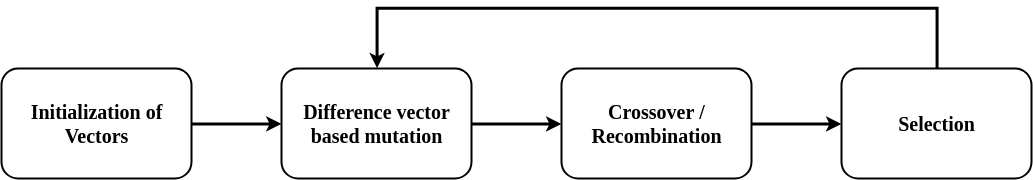
\includegraphics[scale=0.3]{DEop.png}
	\caption{The optimization process of DE \cite{das2011differential}.}\label{img:DE}
\end{figure}

The optimization process of DE the works through a simple cycle of stages, presented in Figure \ref{img:DE}, that we can summarize as follows:

\begin{itemize}
	
	\item \textbf{Initialization of Vectors}: DE begins with a randomly initialized population of a given number of $v$-dimensional arrays of parameters. These vectors constitute candidate solutions for the problem to be solved.
	
	\item \textbf{Difference-vector-based mutation}: DE introduces diversity into the population via the mutation operator. This operator is applied to each individual of the population, known in this context as the parent vector. It combines the parent vector with two randomly selected vectors from the population by applying an arithmetic operator to them. The result of this process is a mutant vector.
	
	\item \textbf{Crossover/Recombination}: The mutant vector exchanges some components with its associated parent to form a trial vector, which will be the candidate to replace the parent vector. Several strategies exist to generate this trial vector, which we will not delve into; however, they can be found in \cite{das2011differential}.
	
	\item \textbf{Selection}: The newly generated trial vector is compared with its associated parent using the fitness function. If the trial vector is better than the parent, then it will replace the parent in the next generation. It is worth noting that, following this strategy, the population never degenerates but only gets better or remains the same.
	
\end{itemize}

Even though DE was a major breakthrough in terms of real optimization, many variants have been developed since its invention that provide better results. We will focus on the SHADE variant, which adaptively optimizes some of the parameters of DE. To carry out this task SHADE uses a historic record of values for these parameters that allows it to set them in favor of the optimization process, based on how good the algorithm behaved with certain parameter values in the past (see Section \ref{sec:SHADE}).



\section{Brief Review of the BRKGA Algorithm} \label{sec:brkga}

Genetic Algorithms (GAs) emerged as one of the first metaheuristics inspired by the concept of natural selection and evolution. It is one of the most studied and successful evolutionary algorithms, thanks in part to its simplicity and ease of implementation \cite{fausto2019ants, goldberg1989genetic}. 

In a GA, a population $P$ of a given number of solutions $p_i = \{p_{[i,1]}, \cdots, p_{[i,v]}\}$ is first initialized; these solutions are also called chromosomes or individuals. Each element of a chromosome is called gene and the value it takes is known as allele. To simulate the natural processes of evolution and natural selection, the set of evolutionary operators that GAs make use of is similar to that used by DE: crossover, mutation and selection. The crossover operator consists in combining two different chromosomes (parents) from the population and obtaining a new chromosome (offspring) which inherits alleles for its genes from both parents. The mutation operator is used by GAs to avoid local optima, and it consists in introducing random changes into the population to favor diversity. The selection operator is used to determine whether a chromosome is suitable to survive for the next generation, and to accomplish this task it employs a fitness function that assigns a value to each chromosome to assess its quality as a solution for the problem. GAs apply these operators through a series of generations to hopefully obtain a solution for the problem to solve that is close to the optimal \cite{fausto2019ants}.  

The Random-Key Genetic Algorithm (RKGA) emerged in \cite{bean1994genetic} as a solid approach to high constrained problems. It uses vectors of random numbers to represent solutions to the problem (individuals), which are used as keys to obtain the actual solutions. Random-key vectors are sampled from the space $[0,1]^{v}$, which is used as a surrogate space for the literal solution space. Points in the random-key space are transferred to the literal solution space via a decoder for fitness evaluation. A decoder is a deterministic procedure that allows us to map random-key vectors to the literal solution space. We can build a decoder that always provides as a result a feasible solution to the problem we want to solve, thus avoiding the feasibility problem that we found in classic GAs.

The Biased Random-key Genetic Algorithm (BRKGA) was first proposed in \cite{gonccalves2011biased} as a variant of the RKGA. In the BRKGA optimization process, first, the population $P$ of $|P|$ vectors of random-keys is initialized; this will be the initial generation. Each random-key vector $p_i$ has $v$ random-keys in it. The population is sorted by the fitness value $f_i$ of each $p_i$ to select the first $P_e$ individuals, this is, the elite of the population. The elite will be preserved in the next generation without modification. To introduce diversity, a number $P_m$ of new random-keys vectors are also included in the next generation. The remaining individuals of the new generation ($|P| - P_e - P_m$) are obtained through crossovers between elite and non-elite parents.

It should be noted that in BRKGA there is a clear differentiation between problem-dependent and problem-independent elements. The independent part of the algorithm has no knowledge of the problem it solves, it is limited to performing the operations related to the population optimization process. The dependent part of the problem is composed of the decoder and the fitness function, which allow us to obtain actual solutions for the problem and its evaluation. Therefore, to specify a BRKGA optimization scheme it is only necessary to define the decoder and the fitness function \cite{gonccalves2011biased}.

\subsection{BRKGA optimization scheme for Constrained Clustering} \label{sec:AdaptationofBRKGA}

An adaptation of BRKGA for constrained clustering was proposed in \cite{de2017comparison}, we will refer to it as BRKGA$_{CC}$.

In this scheme each random-key vector has $n$ random-keys in it ($v = n$). The decoder divides the interval $[0,1]$ in $k$ intervals, so there exists a correspondence between each random-key (instance $x_i$) and the integer (label $l_i$) corresponding to the interval which it lies in. Table \ref{tab:decodingrk} shows an example of random-key decoding for a dataset with 10 instances ($n$ = 10) and $k = 3$. Note that extreme values 0 and 1 can also appear in a random-key vector.

\begin{table}[!h]
	\centering
	%\setlength{\arrayrulewidth}{1mm}
	\setlength{\tabcolsep}{7pt}
	\renewcommand{\arraystretch}{1.2}
	\resizebox{\textwidth}{!}{
	\begin{tabular}{|c|c|c|c|c|c|c|c|c|c|c|}
		\hline
		Index (instance) & 1 & 2 & 3 & 4 & 5 & 6 & 7 & 8 & 9 & 10 \\
		\hline
		Random-key & 0.12 & 0.37 & 0.66 & 0.56 & 0.00 & 0.97 & 0.23 & 0.25 & 0.15 & 1.00 \\
		\hline
		Cluster (label) & 1 & 2 & 2 & 2 & 1 & 3 & 1 & 3 & 1 & 3 \\
		\hline

	\end{tabular}}
	\caption{Random-key decodification example \cite{de2017comparison}.}
	\label{tab:decodingrk}
\end{table}

Once the decoded solution has been obtained, the fitness value of the solution is computed as in Equation \eqref{eq1}.

\begin{equation}
f_i = z_i + \overbrace{(\mu * n * \text{infeasibility}_i)}^\text{penalty},
\label{eq1}
\end{equation}

\noindent where $\mu$ is a high value, $\text{infeasibility}_i$ is the number of non-satisfied constraints and $z_i$ is the within-cluster-sum-of-squares which can be computed as in Equation \eqref{eq2}.

\begin{equation}
z_i = \sum_{c_j \in C_i} \left[ \frac{\sum_{x_a, x_b \in c_j} d^2(x_a,x_b)}{|c_j|}\right],
\label{eq2}
\end{equation}

\noindent where $C_i$ is the partition of dataset $X$ defined by solution (individual) $p_i$, and $(x_a, x_b)$ are instances in the cluster $c_j$ such that $a \neq b$ and the Euclidean distance ($d^2(\cdot, \cdot)$) between each pair of instances in $C_i$ is included in the sum only once.

In \cite{de2017comparison}, the authors also added a new element to BRKGA, a local search procedure. This local optimization method is applied to each decoded individual in each generation, but its results are not transferred to the individual, so that diversity is maintained. Thus, the individuals produced by the local search are only used to update the best solution found so far if needed. For more details on BRKGA$_{CC}$ see \cite{de2017comparison}.

\section{The SHADE Optimization Method} \label{sec:SHADE}

Success History Based Adaptive Differential Evolution (SHADE) is an optimization method based on differential evolution. Proposed in \cite{tanabe2013success}, it was an improvement for the JADE model, presented in \cite{zhang2009jade}.

Unlike JADE, which only considers the parameters used in the previous generation, SHADE uses a historical record of successful parameters as a mechanism for adapting parameters involved in the process of creating new generations.

Since SHADE is an evolution-based algorithm, it shares elements with BRKGA (Section \ref{sec:brkga}), so we will use a similar notation to define its elements. We will note the population as $P_G$, formed by $|P|$ individuals with the form $p_{[i,G]} = \{p_{[i,G,1]}, \cdots, p_{[i,G,v]}\}$, with $G$ indicating the generation to which $p_i$ belongs.

\subsection{SHADE Operators}

As in differential evolution, SHADE employs mutant generation, crossover and selection operators to explore the space of solutions and bring in new generations of individuals.

The mutation strategy used by SHADE is known as current-to-$p$best/1, and the expression that generates new individuals is described in Equation \eqref{eq3}.

\begin{equation}
m_{[i,G]} = p_{[i,G]} + F_i * (p_{[p\text{best}, G]} - p_{[i,G]}) + F_i * (p_{[r1, G]} - p_{[r2,G]}),
\label{eq3}
\end{equation}

\noindent where $m_{[i,G]}$ is the mutant vector, which is generated with an individual $p_{[i,G]}$ from the population serving as a starting point. Indices $r1$ and $r2$ are random values in the range $[0,|P|]$, different from $i$ and from each other. The individual $p_{[p\text{best}, G]}$ is randomly selected from among the best $|P| \times p\text{best}\;|\;p\text{best}\in [0,1]$ individuals in the population. This way, the parameter $p\text{best}$ controls the greediness of the mutation strategy. The parameter $F_i$ defines the magnitude of the operator.

After generating the mutant vector $m_{[i,G]}$, it is combined with the parent $p_{[i,G]}$ vector by means of a crossover operator; the result is the trial vector $t_{[i,G]} = \{t_{[i,G,1]}, \cdots, t_{[i,G,v]}\}$. SHADE uses the Binomial crossover operator, which is defined by the Equation \eqref{eq4}.

\begin{equation}
t_{[i,G,j]} = \left\{ \begin{array}{lc}
m_{[i,G,j]} &   \text{if} \;\; \text{rand}[0,1) \le CR_i \;\; \text{or} \;\;j = j_{rand} \\
p_{[i,G,j]} &  \text{otherwise}
\end{array}
\right.,
\label{eq4}
\end{equation}

\noindent where $\text{rand}[0,1)$ is a random number selected from a normal distribution in the range $[0,1)$, $j_\text{rand}$ is a random integer selected from the range $[1,v]$, and $CR \in [0,1]$ is the crossover ratio.

The SHADE selection operator determines the survivors individuals for the next generation. It compares each parent $x_{[i,G]}$ with the trial vector $t_{[i,G,j]}$, generated based on it. The best one of these two individuals will survive for the next generation. Equation \eqref{eq5} shows this concept.

\begin{equation}
p_{[i,G + 1]} = \left\{ \begin{array}{lc}
t_{[i,G]} &   \text{if} \;\; f(t_{[i,G]}) \le f(p_{[i,G]}) \\
p_{[i,G]} &  \text{otherwise}
\end{array}
\right..
\label{eq5}
\end{equation}

To maintain diversity, SHADE can make use of an external archive $A$, in which parents $p_{[i,G]}$ who were replaced by their associated trial vector $t_{[i,G]}$ are saved. To make use of the archive, we will consider that the individual $p_{[r2,G]}$ from Equation \eqref{eq3} is selected from $P \cup A$. The archive size is the same as the population size. When the size of $A$ exceeds the size of $P$, random individuals are selected for removal to make room for new ones.

The parameters $p\text{best}$, $F_i$ and $CR_i$ are difficult to adjust and their selection is not trivial, as they largely determine the success of the optimization process. These are the parameters that SHADE adaptively optimizes using the mentioned history record.

\subsection{SHADE Parameter Adaptation Method}

The SHADE method stores in memory a structure $M$ with $|M|$ entries for parameters $F_i$ and $CR_i$, as shown in Table \ref{tab:SHADEmemory}. This structure is initialized with the value $0.5$ for all entries.

\begin{table}[!h]
	\centering
	%\setlength{\arrayrulewidth}{1mm}
	\setlength{\tabcolsep}{13pt}
	%\renewcommand{\arraystretch}{0.9}
	\resizebox{\textwidth}{!}{
	\begin{tabular}{|c|c|c|c|c|c|}
		\hline
		 Index & 1 & 2 & $\cdots$ & $|M| - 1$ & $|M|$ \\
		 \hline
		 \hline
		 $M_{CR}$ & $M_{[CR,1]}$ & $M_{[CR,1]}$ & $\cdots$ & $M_{[CR,|M|-1]}$ & $M_{[CR,|M|]}$ \\
		 \hline
		 $M_{F}$ & $M_{[F,1]}$ & $M_{[F,1]}$ & $\cdots$ & $M_{[F,|M|-1]}$ & $M_{[F,|M|]}$ \\
		\hline

	\end{tabular}}
	\caption{Historical memory $M_{CR}$, $M_{F}$ used by SHADE \cite{tanabe2013success}.}
	\label{tab:SHADEmemory}
\end{table}

In each generation, parameters $CR_i$ and $F_i$ are calculated on the basis of the existing history by applying Equations \eqref{eq6} and \eqref{eq7}:

\begin{equation}
CR_i = \text{randn}_i(M_{[CR,r_i]}, 0.1),
\label{eq6}
\end{equation}

\begin{equation}
F_i = \text{randc}_i(M_{[F,r_i]}, 0.1),
\label{eq7}
\end{equation}

\noindent where $\text{randn}(\mu, \sigma^2)$ and $\text{randc}(\mu, \sigma^2)$ are random values from normal and Cauchy distributions respectively, with mean $\mu$ and variance $\sigma^2$. When a value for $CR_i$ outside of the range $[0,1]$ is generated, it is replaced by the corresponding limit value. If $F_i > 1$, then it is truncated to $1$; conversely, if $F_i < 0$, then Equation \eqref{eq7} is applied as many times as needed to obtain a legal value.

SHADE keeps two auxiliary sets $S_{CR}$ and $S_F$ to store the $CR_i$ and $F_i$ values that were successfully used to generate a trial vector that replaced the parent. At the end of each generation, the content of the memory $M$ is updated following Equations \eqref{eq8} and \eqref{eq9}.

\begin{equation}
M_{[CR,h,G+1]} = \left\{ \begin{array}{lc}
\text{mean}_{WA} (S_{CR}) & \text{if} \;\; S_{CR} \neq \emptyset \\
M_{[CR,h,G]} &  \text{otherwise}
\end{array}
\right.,
\label{eq8}
\end{equation}

\begin{equation}
M_{[F,h,G+1]} = \left\{ \begin{array}{lc}
\text{mean}_{WL} (S_{F}) & \text{if} \;\; S_{F} \neq \emptyset \\
M_{[F,h,G]} &  \text{otherwise}
\end{array}
\right..
\label{eq9}
\end{equation}

The $h \;\; (0 \le h \le |M|)$ index specifies the position of the memory $M$ to be updated. This index is initialized to $0$ at the beginning of the optimization process and increased by one after every generation. When $h \ge |M|$ then $h$ is reset to 1. It is worth noting that, when there is a generation with no trial vectors successfully replacing their parents, no update of $M$ is done.

In Equation \ref{eq8}, the term $\text{mean}_{WA} (S_{CR})$ is the weighted mean, which is computed following Equations \eqref{eq10} and \eqref{eq11}, proposed in \cite{peng2009multi} to prevent $CR$ from converging to small values.

\begin{equation}
\text{mean}_{WA} (S_{CR}) = \sum_{i = 1}^{|S_{RC}|} \omega_i * S_{[RC,i]},
\label{eq10}
\end{equation}

\begin{equation}
\omega_i = \frac{\Delta f_i}{\sum_{i = 1}^{|S_{RC}|} \Delta f_i},
\label{eq11}
\end{equation}

\noindent where $\Delta f_i = |f(t_{[i,G]}) - f(p_{[i, G]})|$, which is the amount of improvement obtained from the trial vector with respect to the parent.

In Equation \ref{eq9} the term $\text{mean}_{WL} (S_{F})$ refers to the weighted Lehmer mean, which is computed as in Equation \eqref{eq12} (proposed in \cite{tanabe2013success}).

\begin{equation}
\text{mean}_{WL} (S_{F}) = \frac{\sum_{i = 1}^{|S_{F}|} \omega_i * S^2_{[F,i]}}{\sum_{i = 1}^{|S_{F}|} \omega_i * S_{[F,i]}}.
\label{eq12}
\end{equation}

Unlike parameters $S_{CR}$ and $S_F$, the parameter $p\text{best}$ from Equation \eqref{eq3}, used to set the greediness of the mutation strategy, is not included in the adaptive optimization process. However, it is not static: it is calculated for every individual $p_i$ of the population following Equation \eqref{eq13}.

\begin{equation}
p\text{best}_i = \text{randn}[2/N, 0.2],
\label{eq13}
\end{equation}

\noindent such that there is always at least two individuals to choose between.

\section{SHADE optimization scheme for constrained clustering} \label{sec:SHADEadapt}

In this section, we present an optimization scheme for the SHADE algorithm when applied to constrained clustering. We will call this new approach $SHADE_{CC}$. To begin with, we will use random-keys to create the individuals of the population; this way, each individual is defined as a vector of $n$ random-keys ($v = n$). Additionally, we will also make use of the initialization method and the decoder found in Section \ref{sec:AdaptationofBRKGA}. However, we propose a new fitness function to evaluate the quality of the individuals of the population, Equation \eqref{eq14}, whose element $z_i$ is obtained as in Equation \eqref{eq2}.

\begin{equation}
f_i = z_i * (\text{infeasibility}_i + 1).
\label{eq14}
\end{equation}

Note that in Equation \eqref{eq14} no parameter is involved that cannot be calculated from the dataset or constraints, whereas in Equation \eqref{eq1} the $\mu$ parameter must be calculated and optimized for each individual problem. Therefore with Equation \eqref{eq14} a better generalization capability is obtained.

We found that with the fitness function defined in \eqref{eq1} there is no competition between the penalty term and the within-cluster-sum-of-squares term, because the penalty is always significantly larger than it or zero. This can bias the exploration of the solution space, restricting it in practice to those that satisfy all the constraints, even if the within-cluster-sum-of-squares is still improvable by moving two instances involved in a constraint to different clusters without violating that constraint.

With Equation \eqref{eq14} we try to find a trade-off between the within-cluster-sum-of-squares and the penalty term, allowing solutions that violate a certain number of constraints to compete with those who violate a smaller number of them but score a better within-cluster-sum-of-squares.

To make these concepts clear we consider a toy dataset and three partitions over it. The dataset from Figure \ref{img:toydatasets} contains 100 instances and a single ML constraint between two instances from the same class. Partitions $C_0$---displaying the true labels---and $C_1$ do not violate the constraint ($\text{infeasibility} = 0$), whereas $C_2$ does violate it ($\text{infeasibility} = 1$). However, $C_2$ shows a possibility, for later iterations, of adding both instances to their nearest cluster while also satisfying the ML constraint.

\begin{figure}[bth]
	\myfloatalign
	{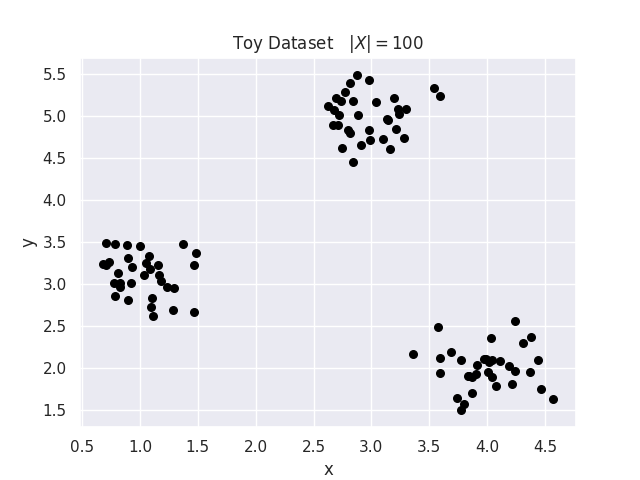
\includegraphics[width=.45\linewidth]{Dataset}} \quad
	%\subfloat[Imagen original]
	{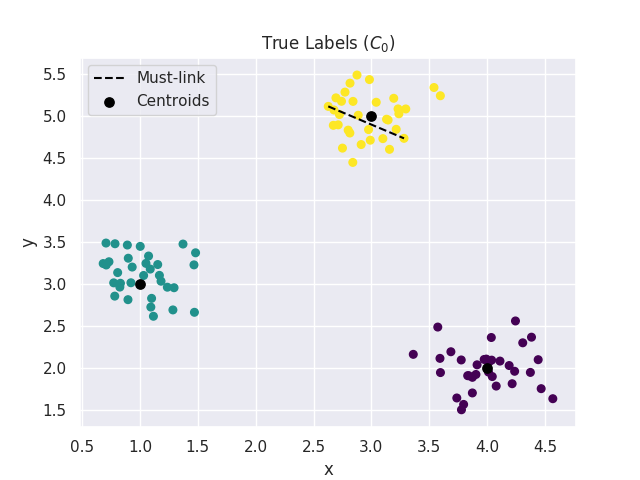
\includegraphics[width=.45\linewidth]{C0}} \quad
	%\subfloat[Clustering sin restricciones]
	{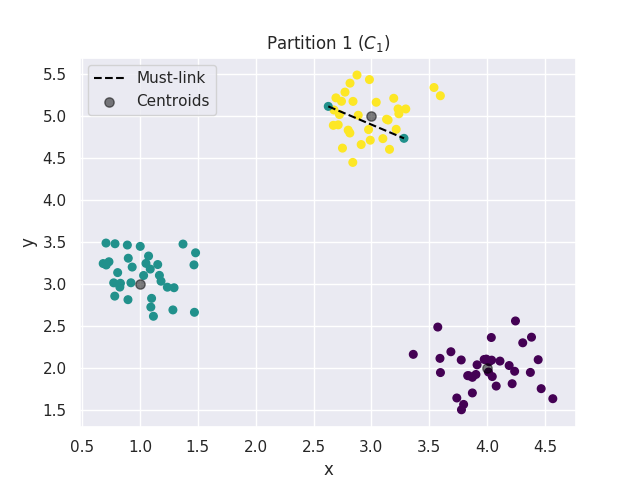
\includegraphics[width=.45\linewidth]{C1}} \quad
	%\subfloat[Clustering con restricciones]
	{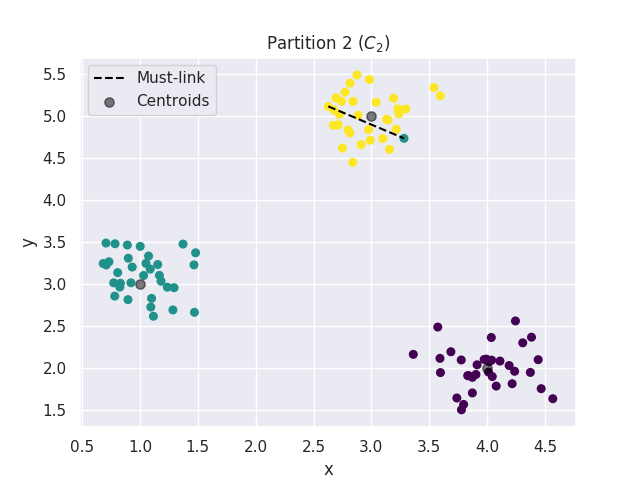
\includegraphics[width=.45\linewidth]{C2}} \quad
	\caption{Three partitions over a toy dataset.}
	\label{img:toydatasets}
\end{figure}

Table \ref{tab:fitnessfunctions} shows the fitness values for each partition from Figure \ref{img:toydatasets}. We refer to the function presented in Equation \eqref{eq1} as $f_1$ and to the function presented in Equation \eqref{eq14} as $f_2$.

\begin{table}[!h]
	\centering
	\setlength{\tabcolsep}{7pt}
	\renewcommand{\arraystretch}{1.3}
	%\begin{adjustwidth}{-1in}{-1in}
	\resizebox{\textwidth}{!}{
		\begin{tabular}{c c c c c c}
			\hline
			\multirow{2}{*}{Partition} &
			\multicolumn{2}{c}{Expression} &&
			\multicolumn{2}{c}{Value} \\
			\cline{2-3} \cline{5-6}
			& $f_1$ & $f_2$ && $f_1$ & $f_2$ \\
			\hline
			$C_0$ & $z_0$ & $z_0$ && $0.457$  & $0.457$  \\
			$C_1$ & $z_1$ & $z_1$ && $0.540$  & $0.540$  \\
			$C_2$ & $z_2 + (\mu * N * \text{infsblt})$ & $z_2 * (\text{infsblt} + 1)$  && $0.503 + 1000 = 1000.503$ &  $0.503 * 2 = 1.005$ \\
			\hline

		\end{tabular}}
		%\end{adjustwidth}

	\caption{Expression and value of fitness functions over three partitions ($\mu = 10$).}
	\label{tab:fitnessfunctions}
\end{table}

Results in Table \ref{tab:fitnessfunctions} are a clear example of the above. In the general case, by using $f_2$ the penalty for violating constraints is proportional to the within-cluster-sum-of-squares---the lower it is, the lower the penalty. This is not the case with $f_1$, whose penalty term is independent of the within-cluster-sum-of-squares, which can result in a difference of several orders of magnitude between partitions satisfying different amounts of constraints.

As in \cite{de2017comparison} we apply a local optimization procedure to the individuals of the population, but without transferring its results to the original individual in order to maintain diversity. The difference is that we do not apply it to the whole population but only to a number $P_e$ of individuals considered as the elite of the population, with the aim of preserving a good exploration-exploitation trade-off. The percentage of individuals considered as elite must be determined for each case.

Algorithm \ref{alg:SHADE} describes the overall SHADE$_{CC}$ optimization process, including the local search procedure presented in Algorithm \ref{alg:LS}. The goal of this procedure is to locally improve solutions (individuals from $P$) in a non-exhaustive way. To do so, it randomly choses an instance from the dataset and iteratively assigns it to different clusters. When improvement in the fitness function is detected, the change is transferred to the solution, when there is no possible improvement the local optimization process stops.

\begin{algorithm}
	\SetNlSty{textbf}{[}{]}
	\SetNlSkip{0.5em}
	\setstretch{1.2}
	\SetKwFunction{Sort}{Sort}
	\SetKwFunction{LocalSearch}{LocalSearch}
	\KwIn{Dataset $X$, constraint sets $C_=$ and $C_{\neq}$, population size $p_{size}$, elite size $P_e$, number of clusters $k$.}
	\tcp{Initialization phase}
	$G \leftarrow 0$\\
	Initialize population $P_0 \leftarrow \{p_{[1,0]}, \cdots, p_{[p_{size},0]}\}$\\
	Initialize all values in $M_{CR}$, $M_F$ to 0.5\\
	$A \leftarrow \emptyset$; $h \leftarrow 1$\\
	\tcp{Main loop}
	\While{Termination criteria are not met}{

		$S_{CR} \leftarrow S_F \leftarrow \emptyset$\\
		$P_G \leftarrow$ \Sort{$P_G$} \tcp{Sort the population}
		\tcp{Apply an LS procedure to the elite of the population}
		\LocalSearch{$\{p_{[1,G]}, \cdots, p_{[p_{e},G]}\}$}\\
		\For{$i \in [1,p_{size}]$}{
			$r_i \leftarrow$ randInt$[1,|M|]$\\
			$CR_{[i,G]} \leftarrow$ randn$_i(M_{[CR,r_i]}, 0.1)$\\
			$F_{[i,G]} \leftarrow$ randc$_i(M_{[F,r_i]}, 0.1)$\\
			$p_{[i,G]} \leftarrow$ rand$[N/2, 0.2]$\\
			\tcp{Generate trial vector $t_{[i,G]}$ by current-to-$p$best/1/bin}

			\eIf{$f(t_{[i,G]}) \le f(p_{[i,G]})$}{
				$p_{[i,G + 1]} \leftarrow t_{[i,G]}$
			}{
				$p_{[i,G + 1]} \leftarrow p_{[i,G]}$
			}

			\If{$f(t_{[i,G]}) < f(p_{[i,G]})$}{
				$p_{[i,G]} \rightarrow A$;
				$CR_{[i,G]} \rightarrow S_{CR}$;
				$F_{[i,G]} \rightarrow S_{F}$
			}

		}
		\tcc{Whenever $|A| > |P|$, randomly select an individual from $A$ to be deleted so that $|A| \le |P|$}
		\If{$S_{CR} \neq \emptyset$ \textbf{and} $S_{F} \neq \emptyset$}{
			Update $M_{[CR,h]}$ and $M_{[F,h]}$ based on $S_{CR}$ and $S_{F}$\\
			$h \leftarrow (h + 1) \mod |M|$
		}
		$G \leftarrow G + 1$
	}
	\caption{SHADE$_{CC}$}\label{alg:SHADE}
\end{algorithm}

\begin{algorithm}
	\SetNlSty{textbf}{[}{]}
	\SetNlSkip{0.5em}
	\setstretch{1.2}
	\SetKwFunction{RandomShuffle}{RandomShuffle}
	\SetKwRepeat{Do}{do}{while}
	\KwIn{Dataset $X$, constraint sets $C_=$ and $C_{\neq}$, decoded random-key vector (solution) $S$, number of clusters $k$.}
	\BlankLine
	\While{$improvement$}{
		$improvement \leftarrow$ \texttt{false} \\

		$s_i \leftarrow $ Select random object from $S$\\
		\tcp{Random shuffle labels set}
		$RSL \leftarrow $ \RandomShuffle{$\{1,\cdots,K\}$}\\
		\For{$l \in RSL$}{
			$S^\prime \leftarrow S$\\
			\tcp{Move object $s_i$ to the cluster associated with label $l$}
			$S^\prime$\texttt{[}$s_i$\texttt{]} $\leftarrow l$\\
			\If{$f(S^\prime) < f(S)$}{
				$S \leftarrow S^\prime$\\
				$improvement \leftarrow$ \texttt{true} \\
			}
		}
	}
	\BlankLine
	\KwRet ($S$)

\caption{Local Search}\label{alg:LS}
\end{algorithm}

\clearpage

\section{Experimental Setup} \label{sec:expSetup}

For our experiments we will compare the results obtained by BRKGA$_{CC}$ and SHADE$_{CC}$ over 25 datasets and 3 constraints set for each one of them. Most of these datasets can be found at the \href{https://sci2s.ugr.es/keel/category.php?cat=clas}{Keel-dataset repository} \cite{triguero2017keel}, though some of them have been obtained via
\href{https://scikit-learn.org/stable/datasets/index.html}{\texttt{scikit-learn} python package} \cite{scikit-learn}. We also include 3 artificial datasets in our analysis, namely: \textit{Circles}, \textit{Moons} and \textit{Spiral}, which can be found at \href{https://github.com/GermangUgr/SHADE_CC}{GitHub}. Table \ref{tab:datasets} displays a summary of every dataset.

\begin{table}[!h]
	\centering
	%\setlength{\arrayrulewidth}{1mm}
	%\setlength{\tabcolsep}{5pt}
	%\renewcommand{\arraystretch}{1.2}
	%\resizebox{\textwidth}{!}{
	\small
	\begin{tabular}{l c c c}
		\hline
		Name & No. Instances & No. Classes & No. Features \\
		\hline
		Appendicitis & 106 & 2 & 7 \\
		Breast Cancer & 569 & 2 & 30 \\
		Bupa & 345 & 2 & 6 \\
		Circles & 300 & 2 & 2 \\
		Ecoli & 336 & 8 & 7 \\
		Glass & 214 & 6 & 9 \\
		Haberman & 306 & 2 & 3 \\
		Hayesroth & 160 & 3 & 4 \\
		Ionosphere & 351 & 2 & 33 \\
		Iris & 150 & 3 & 4 \\
		Led7Digit & 500 & 10 & 7 \\
		Monk2 & 432 & 2 & 6 \\
		Moons & 300 & 2 & 2 \\
		Movement Libras & 360 & 15 & 90 \\
		Pima & 768 & 2 & 8 \\
		Saheart & 462 & 2 & 9 \\
		Sonar & 208 & 2 & 60 \\
		Soybean & 47 & 4 & 35 \\
		Spectfheart & 267 & 2 & 44 \\
		Spiral & 300 & 2 & 2 \\
		Tae & 151 & 3 & 5 \\
		Vehicle & 846 & 4 & 18 \\
		Vowel & 990 & 11 & 13 \\
		Wdbc & 569 & 2 & 30 \\
		Zoo & 101 & 7 & 16 \\
		\hline

	\end{tabular}%}
	\caption{Summary of datasets used for the experiments.}
	\label{tab:datasets}
\end{table}

Classification datasets are commonly used in the literature to test constrained clustering algorithms; they enable us to generate constraints with respect to the true labels (see Section \ref{sec:ConstGent}). They also facilitate an easy evaluation of the quality of the algorithm by means of measures like the Adjusted Rand Index (see Section \ref{sec:EvalMet}).

\subsection{Constraint Generation} \label{sec:ConstGent}

Since we have the true labels associated with each dataset, we will use the method proposed in \cite{wagstaff2001constrained} to generate artificial constraint sets. This method consists of randomly selecting two instances of a dataset, then comparing its labels, and finally setting an ML or CL constraint depending on whether the labels are the same or different.

We will generate, for each dataset, three different sets of constraints---$CS_{10}$, $CS_{15}$ and $CS_{20}$---that will be associated with three small percentages of the size of the dataset: 10\%, 15\% and 20\%. With $n_f$ being the fraction of the size of the dataset associated with each of these percentages, the formula $\frac{n_f(n_f-1)}{2}$ tells us how many artificial constraints will be created for each constraint set; this number is equivalent to how many edges a complete graph with $n_f$ vertices would have.

The random allocation of constraints has a potential advantage over simply using the constraints contained in an $n_f$-vertex complete graph: there is a lower probability of biasing the constraint set towards having classes with poor representation in it. Table \ref{tab:constraints} shows the number of constraints of each type obtained for each dataset.

\begin{table}[!h]
	\centering
	\setlength{\tabcolsep}{7pt}
	\renewcommand{\arraystretch}{1.2}
	%\begin{adjustwidth}{-1in}{-1in}
	\resizebox{\textwidth}{!}{
	\begin{tabular}{lcc c cc c cc}
		\hline
		\multirow{2}{*}{Dataset} &
		\multicolumn{2}{c}{$CS_{10}$} && \multicolumn{2}{c}{$CS_{15}$} && \multicolumn{2}{c}{$CS_{20}$} \\
		\cline{2-3} \cline{5-6} \cline{8-9}
		& ML & CL && ML & CL && ML & CL \\
		\hline
		Appendicitis & 39 & 16 && 71 & 49 && 164 & 67 \\
		Breast Cancer & 876 & 720 && 1965 & 1690 && 3487 & 2954 \\
		Bupa & 323 & 272 && 699 & 627 && 1201 & 1145 \\
		Circles & 208 & 227 && 502 & 488 && 853 & 917 \\
		Ecoli & 163 & 398 && 357 & 918 && 609 & 1669 \\
		Glass & 52 & 179 && 139 & 389 && 259 & 644 \\
		Haberman & 304 & 161 && 634 & 401 && 1135 & 756 \\
		Hayesroth & 39 & 81 && 102 & 174 && 177 & 319 \\
		Ionosphere & 330 & 300 && 732 & 646 && 1299 & 1186 \\
		Iris & 26 & 79 && 82 & 171 && 136 & 299 \\
		Led7Digit & 126 & 1099 && 267 & 2508 && 460 & 4490 \\
		Monk2 & 473 & 473 && 979 & 1101 && 1917 & 1824 \\
		Moons & 200 & 235 && 494 & 496 && 900 & 870 \\
		Movement Libras & 27 & 603 && 112 & 1319 && 158 & 2398 \\
		Pima & 1604 & 1322 && 3595 & 3075 && 6452 & 5329 \\
		Saheart & 595 & 486 && 1292 & 1123 && 2330 & 1948 \\
		Sonar & 100 & 110 && 245 & 251 && 436 & 425 \\
		Soybean & 4 & 6 && 6 & 22 && 12 & 33 \\
		Spectfheart & 233 & 118 && 543 & 277 && 965 & 466 \\
		Spiral & 224 & 211 && 487 & 503 && 918 & 852 \\
		Tae & 40 & 80 && 82 & 171 && 151 & 314 \\
		Vehicle & 874 & 2696 && 1955 & 6046 && 3589 & 10776 \\
		Vowel & 445 & 4406 && 1026 & 10000 && 1705 & 17798 \\
		Wdbc & 840 & 756 && 1925 & 1730 && 3472 & 2969 \\
		Zoo & 21 & 34 && 29 & 91 && 41 & 169 \\
		\hline

	\end{tabular}}
	%\end{adjustwidth}

	\caption{Number of constraints used in experiments.}
	\label{tab:constraints}
\end{table}

Note that the greater the number of classes in the dataset, the fewer ML constraints obtained with the method proposed in \cite{wagstaff2001constrained}. This is because the probability of randomly choosing two individuals from the same class decreases as the number of classes present in the dataset increases.

\clearpage

\subsection{Evaluation Method} \label{sec:EvalMet}

Since we have the true labels associated to each of the datasets, we can use them to evaluate the results provided by each method. We will use the Adjusted Rand Index (ARI) to measure the accuracy of the predictions resulting from each method we test \cite{hubert1985comparing}. The basic Rand Index computes the degree of agreement between two partitions $C_1$ and $C_2$ of a given dataset $X$. $C_1$ and $C_2$ are viewed as collections of $n(n - 1)/2$ pairwise decisions \cite{rand1971objective}.

For each pair of instances $x_i$ and $x_j$ in $X$, a partition assigns them to the same cluster or to different clusters. We take $a$ as the number of pairings where $x_i$ is in the same cluster as $x_j$ in both $C_1$ and $C_2$, and $b$ as the opposite event ($x_i$ and $x_j$ are in different clusters in $C_1$ and $C_2$). Then, the degree of similarity between $C_1$ and $C_2$ is calculated as in Equation \eqref{eq15}.

\begin{equation}
\text{Rand}(C_1, C_2) = \frac{a + b}{n(n - 1)/2}
\label{eq15}
\end{equation}

The ARI is a corrected-for-chance version of the Rand Index. This correction uses the expected similarity of all comparisons between clusterings specified by a random model to set up a baseline. The ARI is computed as in Equation \eqref{eq16}.

\begin{equation}
\text{ARI}(C_1, C_2) = \frac{\text{Rand}(C_1, C_2) - \text{Expected Index}}{\text{Maximum Index} - \text{Expected Index}},
\label{eq16}
\end{equation}

\noindent where Maximum Index is expected to be 1 and Expected Index is the already mentioned expected degree of similarity with a random model. It is easy to see that $\text{ARI}(C_1, C_2) \in [-1,1]$, such that an ARI value close to 1 means a high degree of agreement between $C_1$ and $C_2$, a positive value close to 0 means no agreement and a value smaller that 0 means that the $\text{Rand}(C_1, C_2)$ is less than expected when comparing with random partitions. To summarize, the higher the ARI, the greater the degree of similarity between $C_1$ and $C_2$. For more details on ARI see \cite{hubert1985comparing}.

Our objective is to quantify the quality of the solutions obtained as a result of the methods presented in this paper. To accomplish this task we just set one of the two partitions given to compute ARI as the ground truth labels.

\subsection{Validation of results} \label{sec:ValidtnMethod}

In order to validate the results which will be presented in Section \ref{sec:results} we will use Bayesian statistical tests, instead of the classic Null Hypothesis Statistical Tests (NHST). In \cite{benavoli2017time} we find an in-depth analysis of the disadvantages of NHST, and a new model is proposed for carrying out comparisons researchers are interested in. \textit{"In a nutshell: NHST do not answer the question we ask"}. To put it clear, the disadvantages of the NHST that the authors highlight in \cite{benavoli2017time} are based on the trap of black-and-white thinking, this is: to reject, or not to reject?

To start with, NHST do not provide us with the probabilities associated to the analyzed hypotheses, and therefore it is not possible to answer the question: what is the probability that two methods are different? Another pitfall of NHST is that, with a sufficiently large number of observations, it is possible to reject almost any hypothesis. This is because the p-value does not allow us to separate between the effective size and the sample size, which is established by the researcher.

Also, NHST do not provide information about the magnitude of the effects and the uncertainty of its estimate. As a consequence, NHST may reject hypotheses despite very small effects, or even if there is significant uncertainty in the magnitude of the effects.

Furthermore, and this is a situation that all researchers have faced, NHST do not provide any information about the null hypothesis! That is: What can we conclude when NHST do not reject the null hypothesis? We can not infer anything since NHST can not provide evidence in its favor.

Finally, there are two other problems that researchers face when performing NHST. The first one is the choice of the significance level $\alpha$, for which there are no objective guidelines despite being critical to the test results. The second one is the need to previously formalize the intentions of the sampling of the results, which are usually fixed a posteriori; this could lead to a misreading of said results.

As shown in \cite{benavoli2017time}, most of these problems can be avoided by using Bayesian tests instead of NHST. In particular we will use the Bayesian sign test, which is the Bayesian version of the frequentist non-parametric sign test. To make use of it we will employ the R package \texttt{rNPBST}, whose documentation and guide can be found in \cite{carrasco2017rnpbst}.

We will use the Bayesian sign test to validate our results, which is based on obtaining the statistical distribution of a certain parameter $\rho$ according to the difference between the results, under the assumption that said distribution is a Dirichlet distribution. To get the distribution of $\rho$ we count the number of times that $A - B < 0$, the number of times where there are no significant differences, and the number of times that $A - B > 0$. In order to identify cases where there are no significant differences, we define the region of practical equivalence (rope) $[r_\text{min}, r_\text{max}]$, so that $P(A \approx B) = P(\rho \in \text{rope})$. Using these results we calculate the weights of the Dirichlet distribution and sample it to get a set of triplets with the following form: 
$$[P(\rho < r_\text{min}) = P(A - B < 0),\;\; P(\rho \in \text{rope}),\;\; P(\rho > r_\text{max}) = P(A - B > 0)]$$

\subsection{Calibration}

Table \ref{tab:params} shows a summary of the parameter setup used for both BRKGA$_{CC}$ and SHADE$_{CC}$ algorithms.

\begin{table}[!h]
	\centering
	\setlength{\tabcolsep}{7pt}
	\renewcommand{\arraystretch}{1.4}
	%\begin{adjustwidth}{-1in}{-1in}
	\resizebox{\textwidth}{!}{
		\begin{tabular}{>{\centering\arraybackslash}c m{5cm} cc}
			\hline
			Parameter & Meaning & BRKGA & SHADE \\
			\hline
			$|P|$ & Population size & 100 & 100 \\
			Evals & Fitness function evaluations & 300000 & 300000 \\
			$P_e$ & Size of the elite set in population & $0.2 * |P|$ & $0.25 * |P|$ \\
			$P_m$ & Number of mutants to be introduced in the population in each generation & $0.2 * |P|$ & - \\
			$p_\text{inherit}$ & Probability that a feature is inherited from an elite parent & $50\%$ & - \\
			$k$ & Output partition number of clusters & \multicolumn{2}{m{4cm}}{No. Classes (Table \ref{tab:datasets})} \\
			\hline

		\end{tabular}}
		%\end{adjustwidth}

	\caption{Parameters setup used for BRKGA and SHADE.}
	\label{tab:params}
\end{table}

In both cases---BRKGA$_{CC}$ and SHADE$_{CC}$---the population size will be 100 individuals, and the stop criterion is given by the number of evaluations of the fitness function, which at most will be 300000. A Python implementation for both algorithms can be found at \href{https://github.com/GermangUgr/SHADE\_CC}{GitHub}

To compare with the state-of-the-art methods mentioned in Section \ref{sec:BackSOTA} we will use the parameters setup shown in Table \ref{tab:paramsSOTA} for the implementation that can be found at \href{https://github.com/GermangUgr/TFG/tree/master/Software}{GitHub}

\begin{table}[!h]
	\centering
	\setlength{\tabcolsep}{7pt}
	\renewcommand{\arraystretch}{1.4}
	%\begin{adjustwidth}{-1in}{-1in}
	\resizebox{\textwidth}{!}{
		\begin{tabular}{>{\centering\arraybackslash}c m{5cm} c}
			\hline
			Common Parameters & Meaning & Value \\
			\hline
			\texttt{max\_iter} & Maximum number of iterations & 300 \\
			$k$ & Output partition number of clusters & No. Classes (Table \ref{tab:datasets}) \\
			\hline
			\hline
			Specific Parameters & \multicolumn{2}{l}{Name and Value} \\
			\hline
			COPKM & \multicolumn{2}{l}{\texttt{tolerance} = $1 * 10^{-4}$; \texttt{init\_mode} = \texttt{``rand''}} \\
			CECM & \multicolumn{2}{l}{$\alpha = 1$, $\rho = 100$, $\xi = 0.5$, \texttt{stop\_threshold} = $1 * 10^{-3}$, \texttt{init\_mode} = \texttt{``rand''}} \\
			LCVQE & \multicolumn{2}{l}{\texttt{initial\_centroids} = $\emptyset$} \\
			RDPM & \multicolumn{2}{l}{$\xi_0 = 0.1$, $\xi_\text{rate} = 1$, $\lambda$ is calculated on the basis of the mean distances in the dataset} \\
			TVClust & \multicolumn{2}{l}{$\alpha_0 = 1.2$, \texttt{stop\_threshold} = $5*10^{-4}$} \\
			\hline
			
		\end{tabular}}
		%\end{adjustwidth}
		
	\caption{Parameters setup used for the state-of-the-art algorithms.}
	\label{tab:paramsSOTA}
\end{table}

Parameter values have been assigned following the guidelines of the original creators of the different proposals. Since the evaluation in the experimental stage makes use of a high number of datasets, tuning each parameter specifically for each dataset is not feasible. Indeed, our goal is not optimization in a case-by-case basis but instead a comparison in the most general scenario possible. Therefore, given that the purpose of this work is to draw a fair comparison between the algorithms and assess their robustness in a common environment with multiple datasets, we have not included a tuning step to maximize any particular performance metric.

\section{Experimental Results} \label{sec:results}

In this section we present Tables from \ref{tab:results10} to \ref{tab:results20SOTA}, which display the results obtained by the methods to be compared for each dataset and constraint set.

Since the methods we are comparing involve non-deterministic procedures, the results may vary from one run to another. To lessen the effect this may have on the results, we will apply each method 5 times to every dataset and constraint set, so that the measures shown in the previously mentioned tables correspond to the average of the 5 runs.

\subsection{Comparing BRKGA$_{CC}$ with SHADE$_{CC}$}

In Tables from \ref{tab:results10} to \ref{tab:results20} the ARI columns shows the Adjusted Rand Index for each case, the Unsat columns displays the percentage of violated constraints and the Time columns shows the time taken for each algorithm to deliver results, measured in seconds.

\begin{table}[!h]
	\centering
	\setlength{\tabcolsep}{7pt}
	\renewcommand{\arraystretch}{1.2}
	%\begin{adjustwidth}{-1in}{-1in}
	\resizebox{\textwidth}{!}{
		\begin{tabular}{l ccc c ccc}
			\hline
			\multirow{2}{*}{Dataset} &
			\multicolumn{3}{c}{BRKGA$_{CC}$} &&  \multicolumn{3}{c}{SHADE$_{CC}$} \\
			\cline{2-4} \cline{6-8}
			& ARI & Unsat(\%) & Time(s) && ARI & Unsat(\%) & Time(s) \\
			\hline
			Appendicitis & 0.022 & 5.454 & 383.642 && \textbf{0.086} & 5.091 & 366.491 \\
			Breast Cancer & \textbf{0.395} & 17.444 & 3651.263 && 0.159 & 22.256 & 3602.665 \\
			Bupa & \textbf{0.281} & 14.151 & 1420.117 && 0.104 & 16.672 & 1409.487 \\
			Circles & \textbf{0.166} & 12.598 & 1077.238 && 0.063 & 14.207 & 1060.787 \\
			Ecoli & 0.009 & 20.321 & 1169.798 && \textbf{0.020} & 12.763 & 1112.981 \\
			Glass & \textbf{0.016} & 8.658 & 735.507 && 0.013 & 4.848 & 694.962 \\
			Haberman & 0.047 & 15.699 & 1155.985 && \textbf{0.084} & 15.441 & 1146.023 \\
			Hayesroth & \textbf{0.027} & 1.500 & 550.117 && 0.025 & 2.000 & 529.424 \\
			Ionosphere & 0.125 & 17.587 & 1894.390 && \textbf{0.332} & 12.603 & 1872.308 \\
			Iris & 0.238 & 0.190 & 505.112 && \textbf{0.342} & 0.000 & 483.584 \\
			Led7Digit & \textbf{0.009} & 11.347 & 1786.943 && 0.004 & 8.866 & 1784.708 \\
			Monk2 & \textbf{0.421} & 14.926 & 1848.543 && 0.270 & 16.385 & 1821.208 \\
			Moons & \textbf{0.277} & 11.816 & 1098.089 && 0.272 & 11.356 & 1075.089 \\
			Movement Libras & \textbf{0.004} & 4.159 & 1508.279 && 0.003 & 3.396 & 1519.185 \\
			Pima & 0.236 & 25.195 & 4072.087 && \textbf{0.275} & 22.468 & 3990.383 \\
			Saheart & 0.147 & 20.555 & 2135.624 && \textbf{0.265} & 16.725 & 2095.554 \\
			Sonar & \textbf{0.124} & 7.619 & 1106.039 && 0.116 & 8.952 & 1081.994 \\
			Soybean & 0.496 & 0.000 & 176.333 && \textbf{0.515} & 0.000 & 151.163 \\
			Spectfheart & 0.334 & 9.573 & 1451.235 && \textbf{0.343} & 8.604 & 1405.243 \\
			Spiral & 0.058 & 15.402 & 1098.622 && \textbf{0.114} & 13.793 & 1099.747 \\
			Tae & 0.018 & 0.833 & 520.855 && \textbf{0.024} & 1.333 & 508.988 \\
			Vehicle & 0.005 & 28.515 & 4366.104 && \textbf{0.006} & 22.151 & 4352.663 \\
			Vowel & \textbf{0.003} & 13.330 & 4245.672 && 0.002 & 11.523 & 4290.154 \\
			Wdbc & \textbf{0.478} & 16.316 & 3596.517 && 0.357 & 17.093 & 3528.029 \\
			Zoo & \textbf{0.105} & 1.091 & 336.345 && 0.098 & 2.182 & 317.674 \\
			\hline
			Mean & \textbf{0.161} & 11.771 & 1675.618 && 0.156 & 10.828 & 1652.02 \\
			\hline

		\end{tabular}}
		%\end{adjustwidth}

	\caption{Experimental results obtained for $CS_{10}$ comparing SHADE$_{CC}$ and BRKGA$_{CC}$.}
	\label{tab:results10}
\end{table}

Table \ref{tab:results10} shows the results for the $SC_{10}$ constraint set. We can note that SHADE$_{CC}$ represents a consistent improvement over BRKGA$_{CC}$ in both Unsat and Time, while in terms of ARI both methods are similar. This is because the penalty applied to the fitness function of both methods has little presence when operating with a small constraint set, and since they are population-based and heuristic-guided methods, they have similar exploration and exploitation capabilities.

\begin{table}[!h]
	\centering
	\setlength{\tabcolsep}{7pt}
	\renewcommand{\arraystretch}{1.2}
	%\begin{adjustwidth}{-1in}{-1in}
	\resizebox{\textwidth}{!}{
		\begin{tabular}{l ccc c ccc}
			\hline
			\multirow{2}{*}{Dataset} &
			\multicolumn{3}{c}{BRKGA$_{CC}$} &&  \multicolumn{3}{c}{SHADE$_{CC}$} \\
			\cline{2-4} \cline{6-8}
			& ARI & Unsat(\%) & Time(s) && ARI & Unsat(\%) & Time(s) \\
			\hline
			Appendicitis & 0.296 & 6.167 & 381.625 && \textbf{0.332} & 5.833 & 362.106 \\
			Breast Cancer & 0.772 & 10.172 & 3854.911 && \textbf{0.911} & 3.310 & 3766.402 \\
			Bupa & \textbf{0.840} & 5.973 & 1463.152 && 0.801 & 5.641 & 1437.639 \\
			Circles & 0.828 & 6.101 & 1136.484 && \textbf{0.982} & 0.404 & 1108.928 \\
			Ecoli & 0.015 & 24.314 & 1200.463 && \textbf{0.025} & 19.090 & 1127.568 \\
			Glass & 0.017 & 17.500 & 745.987 && \textbf{0.031} & 11.743 & 722.009 \\
			Haberman & \textbf{0.866} & 4.677 & 1209.471 && 0.796 & 5.314 & 1147.479 \\
			Hayesroth & \textbf{0.107} & 7.536 & 545.861 && 0.099 & 8.261 & 520.702 \\
			Ionosphere & \textbf{0.803} & 7.722 & 1986.543 && 0.591 & 11.974 & 1944.085 \\
			Iris & \textbf{0.412} & 3.873 & 506.548 && 0.260 & 6.087 & 486.723 \\
			Led7Digit & 0.004 & 12.836 & 1902.272 && \textbf{0.007} & 10.919 & 1897.511 \\
			Monk2 & 0.751 & 10.827 & 1949.305 && \textbf{0.945} & 2.067 & 1920.361 \\
			Moons & 0.958 & 1.334 & 1133.858 && \textbf{0.995} & 0.020 & 1113.687 \\
			Movement Libras & \textbf{0.006} & 8.679 & 1584.028 && 0.001 & 8.889 & 1590.321 \\
			Pima & 0.481 & 22.051 & 4451.193 && \textbf{0.762} & 9.928 & 4402.693 \\
			Saheart & 0.749 & 10.940 & 2281.992 && \textbf{0.945} & 1.839 & 2225.210 \\
			Sonar & 0.800 & 5.040 & 1124.700 && \textbf{0.890} & 2.177 & 1069.862 \\
			Soybean & \textbf{0.428} & 0.000 & 170.674 && 0.422 & 0.000 & 155.948 \\
			Spectfheart & \textbf{0.924} & 2.854 & 1561.040 && 0.778 & 5.732 & 1485.260 \\
			Spiral & 0.847 & 5.677 & 1133.962 && \textbf{0.949} & 1.495 & 1102.920 \\
			Tae & \textbf{0.119} & 7.115 & 522.088 && 0.066 & 8.380 & 513.289 \\
			Vehicle & \textbf{0.089} & 28.044 & 4806.559 && 0.018 & 26.856 & 4749.812 \\
			Vowel & \textbf{0.002} & 14.486 & 4807.165 && 0.001 & 13.341 & 4867.849 \\
			Wdbc & 0.805 & 8.985 & 3829.407 && \textbf{0.930} & 2.801 & 3750.711 \\
			Zoo & \textbf{0.157} & 3.500 & 333.984 && 0.128 & 2.834 & 315.131 \\
			\hline
			Mean & 0.483 & 9.456 & 1784.931 && \textbf{0.507} & 6.997 & 1751.368 \\
			\hline

		\end{tabular}}
		%\end{adjustwidth}

	\caption{Experimental results obtained for $CS_{15}$ comparing SHADE$_{CC}$ and BRKGA$_{CC}$.}
	\label{tab:results15}
\end{table}

Table \ref{tab:results15} presents the results obtained with the $CS_{15}$ constraint set. While conclusions for Unsat and Time remain unchanged, we see a clear difference as far as ARI is concerned. We observe that both methods already report ARI results above 0.7, which in an ARI ranking is considered to be an acceptable result. We can even observe that the SHADE$_{CC}$ method provides an ARI higher than 0.9 for 7 datasets, compared to BRKGA$_{CC}$ that only obtains similar results in 2 datasets.

\begin{table}[!h]
	\centering
	\setlength{\tabcolsep}{7pt}
	\renewcommand{\arraystretch}{1.2}
	%\begin{adjustwidth}{-1in}{-1in}
	\resizebox{\textwidth}{!}{
		\begin{tabular}{l ccc c ccc}
			\hline
			\multirow{2}{*}{Dataset} &
			\multicolumn{3}{c}{BRKGA$_{CC}$} &&  \multicolumn{3}{c}{SHADE$_{CC}$} \\
			\cline{2-4} \cline{6-8}
			& ARI & Unsat(\%) & Time(s) && ARI & Unsat(\%) & Time(s) \\
			\hline
			Breast Cancer & 0.807 & 9.086 & 4061.162 && \textbf{0.977} & 0.891 & 3984.370 \\
			Bupa & 0.936 & 2.975 & 1529.151 && \textbf{0.993} & 0.281 & 1508.772 \\
			Circles & 0.935 & 2.814 & 1180.268 && \textbf{1.000} & 0.000 & 1170.452 \\
			Ecoli & 0.028 & 25.716 & 1267.419 && \textbf{0.047} & 21.466 & 1277.903 \\
			Glass & 0.038 & 23.610 & 766.861 && \textbf{0.082} & 16.412 & 796.162 \\
			Haberman & 0.943 & 2.073 & 1266.131 && \textbf{0.997} & 0.138 & 1235.441 \\
			Hayesroth & \textbf{0.548} & 6.331 & 554.339 && 0.531 & 7.056 & 540.585 \\
			Ionosphere & 0.902 & 4.314 & 2051.251 && \textbf{0.993} & 0.258 & 2019.558 \\
			Iris & \textbf{0.691} & 5.241 & 513.675 && 0.553 & 6.528 & 488.262 \\
			Led7Digit & \textbf{0.007} & 13.653 & 2053.264 && 0.005 & 12.170 & 2066.223 \\
			Monk2 & 0.855 & 6.025 & 2055.425 && \textbf{0.991} & 0.379 & 2013.468 \\
			Moons & 0.937 & 2.689 & 1177.848 && \textbf{0.995} & 0.158 & 1157.222 \\
			Movement Libras & \textbf{0.006} & 8.381 & 1654.159 && 0.004 & 7.676 & 1645.174 \\
			Pima & 0.753 & 11.544 & 4855.446 && \textbf{0.899} & 4.419 & 4820.684 \\
			Saheart & 0.881 & 5.250 & 2402.513 && \textbf{0.981} & 0.706 & 2353.931 \\
			Sonar & 0.992 & 0.186 & 1138.769 && \textbf{1.000} & 0.000 & 1127.020 \\
			Soybean & 0.416 & 0.000 & 171.281 && \textbf{0.563} & 0.000 & 153.406 \\
			Spectfheart & 0.953 & 1.677 & 1602.229 && \textbf{1.000} & 0.000 & 1526.925 \\
			Spiral & 0.921 & 3.604 & 1178.580 && \textbf{0.998} & 0.091 & 1155.194 \\
			Tae & 0.351 & 9.807 & 527.292 && \textbf{0.392} & 9.419 & 508.610 \\
			Vehicle & \textbf{0.144} & 28.781 & 5189.066 && 0.044 & 29.008 & 5284.288 \\
			Vowel & 0.002 & 14.682 & 5450.331 && \textbf{0.003} & 13.766 & 5514.052 \\
			Wdbc & 0.823 & 8.281 & 4019.683 && \textbf{0.972} & 1.068 & 3983.564 \\
			Zoo & \textbf{0.176} & 5.429 & 335.715 && 0.153 & 4.191 & 320.186 \\
			\hline
			Mean & 0.602 & 8.086 & 1895.671 && \textbf{0.647} & 5.443 & 1880.921 \\
			\hline

		\end{tabular}}
		%\end{adjustwidth}

	\caption{Experimental results obtained for $CS_{20}$ comparing SHADE$_{CC}$ and BRKGA$_{CC}$.}
	\label{tab:results20}
\end{table}

It is in Table \ref{tab:results20}, which gathers results obtained for the constraint set $CS_{20}$, that we observe major differences between the two methods. We find that SHADE$_{CC}$ is capable of producing clusters identical to the original ones for 4 datasets, regardless the single dataset for which BRKGA$_{CC}$ achieves it. Let us remember that an ARI of 1 represents a perfect match between the two partitions given to compute it. This improvement in ARI is clearly reflected in the percentage of violated constraints---Unsat column---, value for which, once again, SHADE$_{CC}$ outperforms BRKGA$_{CC}$. Conclusions on execution time remain the same.

\subsection{Comparing SHADE$_{CC}$ with the state-of-the-art} \label{sec:SHADEvsSOTA}

In this section we present a brief comparison between the proposed SHADE$_{CC}$ method and some of the state-of-the-art methods. Tables from \ref{tab:results10SOTA} to \ref{tab:results20SOTA} show the results obtained by these methods. To shorten the presented results this time we will only compare the ARI.

It should be noted that there are some missing results in these tables. In the case of the COPKM algorithm, this is due to the fact that it is highly dependent on the order in which constraints are analyzed. It is possible that COPKM cannot find a solution, even though it is always feasible, since the constraints have been generated based on the true labels. In the case of CECM, some of the results are not available because the memory structures that hold the algorithm grow non-linearly with the number of classes and the number of features of the dataset to be analyzed.
	
\begin{table}[!h]
	\centering
	\setlength{\tabcolsep}{7pt}
	\renewcommand{\arraystretch}{1.2}
	%\begin{adjustwidth}{-1in}{-1in}
	\resizebox{\textwidth}{!}{
		\begin{tabular}{lcccccc}
			\hline
			Dataset & SHADE$_{CC}$ & COPKM & LCVQE & RDPM & TVClust & CECM \\
			\hline
			Appendicitis & 0.086 & - & \textbf{0.335} & 0.316 & 0.025 & -0.005 \\
			Breast Cancer & 0.159 & -0.604 & 0.486 & \textbf{0.502} & 0.000 & 0.000 \\
			Bupa & \textbf{0.104} & - & -0.005 & -0.005 & -0.004 & -0.011 \\
			Circles & 0.063 & - & -0.003 & \textbf{0.162} & 0.137 & 0.133 \\
			Ecoli & 0.020 & - & 0.387 & \textbf{0.417} & 0.265 & - \\
			Glass & 0.013 & 0.184 & \textbf{0.268} & 0.197 & 0.211 & - \\
			Haberman & 0.084 & - & -0.002 & 0.127 & \textbf{0.218} & -0.004 \\
			Hayesroth & 0.025 & - & 0.106 & 0.097 & 0.054 & \textbf{0.139} \\
			Ionosphere & \textbf{0.332} & - & 0.168 & 0.197 & 0.000 & 0.030 \\
			Iris & 0.342 & -0.285 & \textbf{0.730} & 0.607 & 0.244 & 0.684 \\
			Led7Digit & 0.004 & \textbf{0.497} & 0.425 & 0.369 & 0.316 & - \\
			Monk2 & 0.270 & \textbf{0.982} & 0.072 & 0.094 & -0.002 & 0.007 \\
			Moons & 0.272 & - & 0.241 & 0.319 & \textbf{0.785} & 0.092 \\
			Movement Libras & 0.003 & 0.285 & \textbf{0.293} & 0.256 & 0.000 & - \\
			Pima & \textbf{0.275} & - & 0.076 & 0.075 & 0.145 & -0.008 \\
			Saheart & 0.265 & \textbf{0.974} & 0.018 & 0.020 & 0.068 & 0.000 \\
			Sonar & \textbf{0.116} & - & 0.004 & 0.013 & 0.000 & 0.000 \\
			Soybean & 0.515 & 0.503 & 0.545 & \textbf{0.621} & 0.000 & 0.244 \\
			Spectfheart & \textbf{0.343} & - & -0.107 & -0.114 & 0.000 & 0.050 \\
			Spiral & \textbf{0.114} & - & -0.003 & 0.012 & 0.034 & -0.002 \\
			Tae & 0.024 & - & 0.009 & -0.000 & \textbf{0.067} & 0.000 \\
			Vehicle & 0.006 & - & 0.121 & 0.081 & \textbf{0.280} & - \\
			Vowel & 0.002 & - & 0.063 & -0.003 & \textbf{0.067} & - \\
			Wdbc & 0.357 & - & 0.486 & \textbf{0.502} & 0.000 & 0.000 \\
			Zoo & 0.098 & \textbf{0.715} & 0.666 & 0.412 & 0.335 & - \\
			\hline
			Mean  & 0.156 & -0.51 & \textbf{0.215} & 0.211 & 0.13 & -0.226 \\
			\hline
		\end{tabular}}
		%\end{adjustwidth}
		
	\caption{Experimental results obtained for $CS_{10}$ comparing SHADE$_{CC}$ and the state-of-the-art.}
	\label{tab:results10SOTA}
\end{table}

Table \ref{tab:results10SOTA} presents the results obtained for the $CS_{10}$ constraint set. LCVQE, RDPM and TVClust methods stand out, achieving results as competitive as SHADE$_{CC}$ with a low number of constraints.

\begin{table}[!h]
	\centering
	\setlength{\tabcolsep}{7pt}
	\renewcommand{\arraystretch}{1.2}
	%\begin{adjustwidth}{-1in}{-1in}
	\resizebox{\textwidth}{!}{
		\begin{tabular}{lcccccc}
			\hline
			Dataset & SHADE$_{CC}$ & COPKM & LCVQE & RDPM & TVClust & CECM \\
			\hline
			Appendicitis & \textbf{0.332} & - & 0.305 & 0.284 & 0.025 & -0.006 \\
			Breast Cancer & 0.911 & \textbf{1.000} & 0.486 & 0.502 & 0.000 & 0.037 \\
			Bupa & 0.801 & \textbf{1.000} & -0.005 & -0.007 & -0.007 & 0.001 \\
			Circles & 0.982 & \textbf{1.000} & -0.003 & 0.375 & 0.973 & 0.105 \\
			Ecoli & 0.025 & - & 0.387 & 0.372 & \textbf{0.719} & - \\
			Glass & 0.031 & - & 0.280 & 0.253 & 0.229 & - \\
			Haberman & 0.796 & \textbf{1.000} & -0.002 & 0.075 & 0.219 & -0.050 \\
			Hayesroth & 0.099 & - & 0.106 & 0.107 & \textbf{0.150} & 0.135 \\
			Ionosphere & 0.591 & \textbf{1.000} & 0.178 & 0.212 & 0.000 & 0.057 \\
			Iris & 0.260 & - & \textbf{0.730} & 0.547 & 0.421 & 0.684 \\
			Led7Digit & 0.007 & - & 0.425 & \textbf{0.490} & 0.324 & - \\
			Monk2 & 0.945 & \textbf{1.000} & 0.072 & 0.170 & -0.002 & 0.007 \\
			Moons & 0.995 & \textbf{1.000} & 0.241 & 0.436 & 0.987 & 0.095 \\
			Movement Libras & 0.001 & -0.742 & \textbf{0.293} & 0.255 & 0.000 & - \\
			Pima & \textbf{0.762} & - & 0.076 & 0.075 & 1.000 & 0.000 \\
			Saheart & 0.945 & \textbf{1.000} & 0.020 & 0.037 & 0.221 & 0.000 \\
			Sonar & \textbf{0.890} & - & 0.004 & 0.019 & 0.000 & 0.000 \\
			Soybean & 0.422 & 0.584 & 0.545 & \textbf{0.605} & 0.000 & 0.000 \\
			Spectfheart & 0.778 & \textbf{0.983} & -0.107 & -0.117 & 0.000 & -0.070 \\
			Spiral & \textbf{0.949} & - & -0.003 & 0.014 & 0.006 & 0.051 \\
			Tae & \textbf{0.066} & - & 0.008 & -0.004 & 0.062 & 0.000 \\
			Vehicle & 0.018 & \textbf{1.000} & 0.121 & 0.081 & 0.576 & - \\
			Vowel & 0.001 & - & 0.063 & -0.003 & \textbf{0.073} & - \\
			Wdbc & 0.930 & \textbf{1.000} & 0.486 & 0.502 & 0.000 & 0.000 \\
			Zoo & 0.128 & 0.435 & \textbf{0.642} & 0.450 & 0.353 & - \\
			\hline
			Mean  & \textbf{0.507} & 0.01 & 0.213 & 0.229 & 0.253 & -0.238 \\
			\hline
		\end{tabular}}
		%\end{adjustwidth}
		
	\caption{Experimental results obtained for $CS_{15}$ comparing SHADE$_{CC}$ and the state-of-the-art.}
	\label{tab:results15SOTA}
\end{table}

In one hand, Table \ref{tab:results15SOTA}, which shows the results for the $CS_{15}$ constraint set, we observe that there is a significant improvement in precision in the results obtained by SHADE$_{CC}$. On the other hand, methods that obtained better results for smaller constraint sets do not present an improvement comparable to that presented by SHADE$_{CC}$, with the exception of COPKM, which is able to reach the optimum for some of the cases in which it finds a solution.

\begin{table}[!h]
	\centering
	\setlength{\tabcolsep}{7pt}
	\renewcommand{\arraystretch}{1.2}
	%\begin{adjustwidth}{-1in}{-1in}
	\resizebox{\textwidth}{!}{
		\begin{tabular}{lcccccc}
			\hline
			Dataset & SHADE$_{CC}$ & COPKM & LCVQE & RDPM & TVClust & CECM \\
			\hline
			Appendicitis & \textbf{1.000} & - & 0.305 & 0.331 & 0.012 & -0.006 \\
			Breast Cancer & 0.977 & \textbf{1.000} & 0.486 & 0.502 & 0.000 & 0.000 \\
			Bupa & 0.993 & \textbf{1.000} & -0.005 & -0.007 & -0.006 & 0.000 \\
			Circles & \textbf{1.000} & \textbf{1.000} & -0.003 & 0.629 & \textbf{1.000} & 0.138 \\
			Ecoli & 0.047 & - & 0.387 & 0.459 & \textbf{0.763} & - \\
			Glass & 0.082 & - & 0.271 & \textbf{0.287} & 0.218 & - \\
			Haberman & 0.997 & \textbf{1.000} & -0.002 & 0.106 & 0.737 & 0.000 \\
			Hayesroth & \textbf{0.531} & - & 0.106 & 0.107 & 0.208 & 0.056 \\
			Ionosphere & 0.993 & \textbf{1.000} & 0.173 & 0.309 & 0.000 & 0.115 \\
			Iris & 0.553 & - & \textbf{0.708} & 0.540 & 0.585 & 0.684 \\
			Led7Digit & 0.005 & - & 0.425 & \textbf{0.571} & 0.327 & - \\
			Monk2 & 0.991 & \textbf{1.000} & 0.072 & 0.253 & -0.002 & 0.160 \\
			Moons & 0.995 & \textbf{1.000} & 0.241 & 0.831 & \textbf{1.000} & 0.180 \\
			Movement Libras & 0.004 & - & \textbf{0.293} & \textbf{0.293} & 0.000 & - \\
			Pima & 0.899 & \textbf{1.000} & 0.076 & 0.076 & \textbf{1.000} & -0.005 \\
			Saheart & 0.981 & \textbf{1.000} & 0.018 & 0.026 & \textbf{1.000} & -0.006 \\
			Sonar & \textbf{1.000} & \textbf{1.000} & 0.004 & 0.127 & 0.000 & 0.003 \\
			Soybean & 0.563 & -0.218 & 0.545 & \textbf{0.631} & 0.000 & -0.016 \\
			Spectfheart & \textbf{1.000} & \textbf{1.000} & -0.107 & -0.112 & 0.000 & -0.054 \\
			Spiral & 0.998 & \textbf{1.000} & -0.003 & 0.011 & 0.006 & 0.045 \\
			Tae & \textbf{0.392} & - & 0.008 & 0.000 & 0.035 & 0.000 \\
			Vehicle & 0.044 & \textbf{1.000} & 0.122 & 0.081 & 0.689 & - \\
			Vowel & 0.003 & - & 0.063 & -0.003 & \textbf{0.071} & - \\
			Wdbc & 0.972 & \textbf{1.000} & 0.486 & 0.522 & 0.000 & 0.000 \\
			Zoo & 0.153 & \textbf{0.821} & 0.642 & 0.439 & 0.335 & - \\
			\hline
			Mean  & \textbf{0.647} & 0.224 & 0.212 & 0.28 & 0.319 & -0.228 \\
			\hline
		\end{tabular}}
		%\end{adjustwidth}
		
	\caption{Experimental results obtained for $CS_{20}$ comparing SHADE$_{CC}$ and the state-of-the-art.}
	\label{tab:results20SOTA}
\end{table}

Table \ref{tab:results20SOTA} presents the results obtained for $CS_{20}$. For SHADE$_{CC}$ we continue to observe its progression in accuracy. As far as the state-of-the-art methods are concerned, we find a general improvement in ARI, except for CECM. Even with this, it is SHADE$_{CC}$ and COPKM that seem to obtain the highest quality results, with the difference that SHADE$_{CC}$ is able to produce results in all cases.

\clearpage

\section{Statistical Analysis of Results} \label{sec:analisis}

With the results obtained by all methods for a total of 75 different datasets---the 25 datasets in combination with the 3 constraint sets for each one of them---we can perform an empirical analysis of them. This way we can statistically determine whether SHADE$_{CC}$ represents a significant improvement over previous proposals.

Having in mind the notation introduced in Section \ref{sec:ValidtnMethod}, and as far as the comparison of population-based methods is concerned, we will refer to the results obtained by BRKGA$_{CC}$ as sample $A$, and to the results obtained with SHADE$_{CC}$ as sample $B$.

One of the major advantages of the Bayesian sign test is that we can obtain a very illustrative visual representation of its results. We can produce a representation of the triplet set in the form of a heatmap where each triplet constitutes one point whose location is given by barycentric coordinates. With this in mind, we will associate each of the triplet values with each of the three vertices of an equilateral triangle. In order to find out where a certain triplet will be placed within the triangle, we will take each of its three values and draw a parallel line to the opposing side of the corresponding vertex; the separation between a triangle side and its parallel line will be proportional to the associated triplet value, so that the higher the value, the closer the line will be to the vertex. The location where the three lines intersect is where we draw a point. Since the values of every triplet describe a probability distribution and therefore they must add up to one, we can be sure that all triplets will lie in some point within the triangle. The color indicates the density of points in a given region, with yellow representing a high density and red a low density.

\begin{figure}[ht!]
	\centering
	\begin{subfigure}{.45\textwidth}
		\includegraphics[width=1\linewidth]{BayesSignoARI.pdf}
		\caption{ARI}
		\label{fig:bayesARI}
	\end{subfigure}
	\begin{subfigure}{.45\textwidth}
		\includegraphics[width=1\linewidth]{BayesSignoTime.pdf}
		\caption{Time}
		\label{fig:bayesTime}
	\end{subfigure}
	\begin{subfigure}{.45\textwidth}
		\includegraphics[width=1\linewidth]{BayesSignoUnsat.pdf}
		\caption{Unsat}
		\label{fig:bayesUnsat}
	\end{subfigure}
	\caption{Heat diagrams for the comparison with BRKGA$_{CC}$.}
\end{figure}

In one hand, figure \ref{fig:bayesARI} shows the heatmap associated with the ARI measurement. The diagram suggests that the Bayesian sign test assigns a high probability to $A - B < 0$, since most triplets are represented in the lower left third of the triangle. It also indicates that in some cases there are no significant differences between $A$ and $B$, since we also find triplets in the rope area. Bearing this in mind, and considering that ARI is a measure to maximize, we can say that, for cases where there are significant differences, SHADE$_{CC}$ performs better than BRKGA$_{CC}$. On the other hand, Figures \ref{fig:bayesTime} and \ref{fig:bayesUnsat} which show the heatmaps obtained for Time and Unsat measurements, are very similar. In both, all triplets are represented in the lower right third of the triangle, indicating that the Bayesian sign test assigns a high probability to $A - B > 0$. With this, and bearing in mind that both measures must be minimized, we conclude that SHADE$_{CC}$ represents a solid improvement over BRKGA$_{CC}$ as far as this measures are concerned.

Regarding the comparison of SHADE$_{CC}$ with the state-of-the-art, we will keep the results obtained by SHADE$_{CC}$ as $B$, and note the results obtained by the state-of-the-art methods as $A$.

This way, we apply the process described earlier in this section to obtain the heatmaps corresponding to the comparison of SHADE$_{CC}$ with each of the 5 state-of-the-art methods. This time the only measure we compare is ARI. Figures \ref{fig:bayesCOPKM} to \ref{fig:bayesCECM} show said comparison.

\begin{figure}[ht!]
	\centering
	\begin{subfigure}{.45\textwidth}
		\includegraphics[width=1\linewidth]{AriCOPKM.pdf}
		\caption{SHADE$_{CC}$ vs COPKM}
		\label{fig:bayesCOPKM}
	\end{subfigure}
	\begin{subfigure}{.45\textwidth}
		\includegraphics[width=1\linewidth]{AriLCVQE.pdf}
		\caption{SHADE$_{CC}$ vs LCVQE}
		\label{fig:bayesLCVQE}
	\end{subfigure}
	\begin{subfigure}{.45\textwidth}
		\includegraphics[width=1\linewidth]{AriRDPM.pdf}
		\caption{SHADE$_{CC}$ vs RDPM}
		\label{fig:bayesRDPM}
	\end{subfigure}
	\begin{subfigure}{.45\textwidth}
		\includegraphics[width=1\linewidth]{AriTVClust.pdf}
		\caption{SHADE$_{CC}$ vs TVClust}
		\label{fig:bayesTVClust}
	\end{subfigure}
	\begin{subfigure}{.45\textwidth}
		\includegraphics[width=1\linewidth]{AriCECM.pdf}
		\caption{SHADE$_{CC}$ vs CECM}
		\label{fig:bayesCECM}
	\end{subfigure}
	\caption{Heat diagrams for the comparison with the state-of-the-art.}
\end{figure}

We see very similar diagrams for COPKM (\ref{fig:bayesCOPKM}), LVCQE (\ref{fig:bayesLCVQE}), RDPM (\ref{fig:bayesRDPM}) and TVClust (\ref{fig:bayesTVClust}). In all of them most of the triplets are represented in the lower middle region of the diagram, with a slight shift of the point cloud to the left. That is indicative that there are indeed significant differences between the two methods---since there are no triplets with representation in the rope area---, but the advantage is for one or the other depending on the case, being SHADE$_{CC}$ the one that gets it in most of them. However, this does not apply in the case of CECM (\ref{fig:bayesCECM}), where the advantage is indisputably for SHADE$_{CC}$.

\section{Conclusions} \label{sec:conclusiones}

In this paper we proposed SHADE$_{CC}$, the first application of a DE-based algorithm to the SSL constrained clustering problem. Focusing on the instance-level ML and CL constraints, SHADE$_{CC}$ has proven that nature-inspired evolution-based techniques constitute a good approach to constrained clustering, being able to scale the quality of the results in a way directly proportional to the number of constraints.
 
Supported by the Bayesian statistical tests, we were able to objectively prove that the SHADE$_{CC}$ approach is significantly better than previous evolution-based proposals. As far as the state-of-the-art is concerned, the SHADE$_{CC}$ approach has proven to be equivalent or better when considering the quality of the solutions, especially in cases where large sets of constraints are analyzed.

\section*{Acknowledgements}

Our work has been supported by the research project TIN2017-89517-P and PP2016.PRI.I.02.

\section*{Compliance with ethical standards}

\section*{Declaration of competing interest}

The authors declare that there is no conflict of interest.

\clearpage

\section*{References}

\bibliography{mybibfile}

\end{document}